\documentclass[aspectratio=169,10pt]{beamer}

\usetheme{default}
\usefonttheme{serif}

\usepackage[T1]{fontenc}
\usepackage[utf8]{inputenc}
\usepackage{mathpazo}
\usepackage{amsmath,amssymb}
\usepackage{booktabs}
\usepackage{xcolor}
\usepackage{tikz}
\usetikzlibrary{arrows.meta,positioning}

\definecolor{cream}{RGB}{248,247,242}
\definecolor{ink}{RGB}{12,12,12}
\definecolor{mid}{RGB}{130,128,122}

\setbeamercolor{background canvas}{bg=cream}
\setbeamercolor{normal text}{fg=ink}
\setbeamercolor{frametitle}{fg=ink,bg=cream}
\setbeamercolor{alerted text}{fg=ink}
\setbeamercolor{structure}{fg=ink}
\setbeamertemplate{navigation symbols}{}
\setbeamertemplate{itemize item}{\textbullet}
\setbeamertemplate{itemize subitem}{-}

\setbeamertemplate{footline}{%
  \hfill\textcolor{mid}{\tiny\insertframenumber\hspace*{0.6cm}\vspace*{0.35cm}}%
}

\setbeamertemplate{frametitle}{%
  \vspace*{0.30cm}%
  \centering{\normalsize\bfseries\insertframetitle}\par%
  \vspace*{0.12cm}%
  \centering\textcolor{mid!60}{\rule{0.30\textwidth}{0.3pt}}\par%
  \vspace*{0.06cm}%
}

\setbeamertemplate{title page}{%
  \centering%
  \vspace*{1.8cm}%
  {\LARGE\bfseries\inserttitle\par}%
  \vspace*{0.9em}%
  {\footnotesize\textcolor{mid}{\MakeUppercase{\insertsubtitle}}\par}%
  \vspace*{2.0em}%
  \textcolor{mid!50}{\rule{0.40\textwidth}{0.3pt}}\par%
  \vspace*{0.9em}%
  {\small\insertauthor\par}%
  \vspace*{0.3em}%
  {\footnotesize\textcolor{mid}{\insertdate}\par}%
}

\title{Cost-Sensitive Predictive Modeling\\for Targeted Marketing Campaigns}
\subtitle{Project 2 \textperiodcentered{} Advanced Machine Learning}
\author{Anna Ostrowska \textperiodcentered{} Gabriela Majstrak \textperiodcentered{} Igor Lechoszest}
\date{Warsaw University of Technology, June 2026}

\newcommand{\sectionslide}[1]{%
  \begin{frame}[plain]
    \centering\vfill
    \textcolor{mid}{\rule{0.10\textwidth}{0.3pt}}\par\vspace{0.5em}
    {\large\bfseries #1}\par\vspace{0.5em}
    \textcolor{mid}{\rule{0.10\textwidth}{0.3pt}}
    \vfill
  \end{frame}%
}

\newcommand{\slabel}[1]{\textbf{\tiny\MakeUppercase{#1}}\\[0.25em]}

\begin{document}

\begin{frame}[plain]
\titlepage
\end{frame}

\begin{frame}{Outline}
\tableofcontents
\end{frame}

% ============================================================================
\section{Problem and Data}
\sectionslide{Problem and Data}
% ============================================================================

\begin{frame}{Business Setup and Scoring Rule}
\begin{columns}[T]
\column{0.54\textwidth}

\slabel{Scenario}
A bank selects up to 1\,000 customers from 5\,000 to contact with a product offer.

\vspace{0.4em}
\begin{tabular}{@{}ll@{}}
  Converts  & \textbf{+10 EUR} \\[0.15em]
  Ignores   & \textbf{$-$5 EUR} \\[0.15em]
  Per variable & \textbf{$-$200 EUR} \\
\end{tabular}

\vspace{0.5em}
\slabel{Break-even threshold}
$\mathbb{E}[\text{gain}\,|\,\hat{p}] = 15\hat{p} - 5 > 0$, so $\hat{p} > \tfrac{1}{3}$

\column{0.42\textwidth}

\slabel{Scoring formula}
\[
  S = 10\cdot\mathrm{TP} - 5\cdot\mathrm{FP} - 200\cdot K
\]
\vspace{0.2em}
{\footnotesize\itshape Each extra variable must generate $>$200 EUR in added profit. Accuracy and profit are decoupled objectives.}

\end{columns}
\end{frame}

\begin{frame}{Dataset and EDA Highlights}
\begin{columns}[T]
\column{0.47\textwidth}

\slabel{Dataset}
\begin{itemize}\itemsep2pt
  \item 5\,000 train + 5\,000 test observations
  \item 500 anonymised features (V1--V500)
  \item Nearly balanced: 49.76\% positives
  \item No missing or constant features
\end{itemize}

\column{0.49\textwidth}

\slabel{Key EDA findings}
\begin{itemize}\itemsep2pt
  \item Weak feature--target correlations ($\rho_{\max}=0.114$, V390)
  \item 23 pairs with $|\rho|>0.80$
  \item Two perfect collinearities:\\
        V32$\equiv$V175, \; V160$\equiv$V416
  \item Including both: $\times$2 cost, 0 gain
\end{itemize}

\end{columns}

\vspace{0.4em}
{\footnotesize\itshape Multivariate model needed, but 200 EUR per variable forces aggressive, profit-aware selection.}
\end{frame}

% ============================================================================
\section{Baseline Methods}
\sectionslide{Baseline Methods}
% ============================================================================

\begin{frame}{Why Standard Feature Selection Fails}
\begin{center}
\footnotesize
\begin{tabular}{@{}lrrrc@{}}
\toprule
Approach & $K$ & Data cost & Val.\ acc. & Profit \\
\midrule
LR, single feature (V390)    & 1  & 200 EUR    & 0.538 & +2\,280 EUR \\
LR, top-5 correlated         & 5  & 1\,000 EUR & 0.578 & +1\,490 EUR \\
LR, Boruta features (26)     & 26 & 5\,200 EUR & 0.605 & $-$2\,730 EUR \\
HGB, Boruta features (26)    & 26 & 5\,200 EUR & \textbf{0.680} & $-$2\,730 EUR \\
LR, L1 regularisation        & 56 & 11\,200 EUR & 0.565 & $-$8\,750 EUR \\
\midrule
\textbf{Proposed pipeline}      & \textbf{4} & \textbf{800 EUR} & \textbf{---} & \textbf{+5\,165 EUR (CV)} \\
\bottomrule
\end{tabular}
\end{center}

\vspace{0.3em}
{\footnotesize\itshape HGB on Boruta features achieves 68\% accuracy (the highest baseline) yet yields $-$2\,730 EUR. The 5\,200 EUR data cost overwhelms the gain. Higher accuracy $\neq$ higher profit.}
\end{frame}

% ============================================================================
\section{Proposed Pipeline}
\sectionslide{Proposed Pipeline}
% ============================================================================

\begin{frame}{Four-Stage Profit-Driven Feature Selector}
\begin{center}
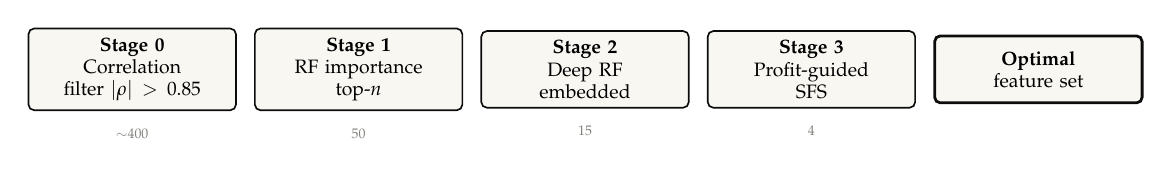
\begin{tikzpicture}[
    node distance=0.25cm and 0.22cm,
    box/.style={draw=ink, rounded corners=2pt, minimum width=2.4cm, minimum height=0.85cm,
                text centered, text width=2.4cm, fill=cream, font=\scriptsize, line width=0.6pt},
    arr/.style={-Stealth, color=mid, thick}
]
\node[box] (s0) {\textbf{Stage 0}\\Correlation\\filter $|\rho|>0.85$};
\node[box, right=of s0] (s1) {\textbf{Stage 1}\\RF importance\\top-$n$};
\node[box, right=of s1] (s2) {\textbf{Stage 2}\\Deep RF\\embedded};
\node[box, right=of s2] (s3) {\textbf{Stage 3}\\Profit-guided\\SFS};
\node[box, right=of s3, line width=1.0pt] (out) {\textbf{Optimal}\\feature set};
\node[below=0.10cm of s0, font=\tiny, color=mid] {$\sim$400};
\node[below=0.10cm of s1, font=\tiny, color=mid] {50};
\node[below=0.10cm of s2, font=\tiny, color=mid] {15};
\node[below=0.10cm of s3, font=\tiny, color=mid] {4};
\end{tikzpicture}
\end{center}

\vspace{0.25em}
\begin{columns}[T]
\column{0.24\textwidth}
{\footnotesize\textbf{Stage 0}}\\\footnotesize
Remove redundant collinear features.
\column{0.24\textwidth}
{\footnotesize\textbf{Stage 1}}\\\footnotesize
Shallow RF, keep top-$n$ by impurity.
\column{0.24\textwidth}
{\footnotesize\textbf{Stage 2}}\\\footnotesize
Deeper RF (300 trees), refined rank.
\column{0.24\textwidth}
{\footnotesize\textbf{Stage 3}}\\\footnotesize
Add feature while CV profit increases.
\end{columns}
\end{frame}

\begin{frame}{Stage 3: Greedy SFS and Threshold Optimisation}
\begin{columns}[T]
\column{0.52\textwidth}

\slabel{Greedy stopping criterion}
Marginal gain of candidate $f$ at step $t$:
\[
  \Delta_t(f) = \hat{S}_{\mathrm{CV}}(\mathcal{F}_t \cup \{f\}) - \hat{S}_{\mathrm{CV}}(\mathcal{F}_t) - 200
\]
Add $\arg\max_f \Delta_t(f)$ if positive, else stop.

\vspace{0.4em}
\slabel{After feature selection}
\begin{itemize}\itemsep2pt
  \item 24-iter randomised HGB search
  \item HGB-only vs.\ ensemble (HGB+RF+LR)\\compared by OOF profit
  \item Threshold grid $[0.15,\,0.50]$, 36 points
\end{itemize}

\column{0.44\textwidth}

\slabel{Why not filter / embedded alone?}
{\footnotesize Filter uses surrogate importance scores. SFS evaluates the actual financial objective with a real classifier, including the 200 EUR marginal cost.}

\vspace{0.5em}
\slabel{Threshold optimisation}
{\footnotesize
\[
  \tau^* = \arg\max_\tau \bigl[10\,\mathrm{TP}(\tau) - 5\,\mathrm{FP}(\tau)\bigr]
\]
Variable cost $200K$ is $\tau$-independent.}

\end{columns}
\end{frame}

% ============================================================================
\section{Experiments}
\sectionslide{Experiments}
% ============================================================================

\begin{frame}{Experiment: Free Feature Engineering}

\slabel{Motivation}
Having paid for $K=6$ variables, generate additional features at zero extra cost.

\vspace{0.3em}
\begin{center}
\footnotesize
\begin{tabular}{@{}lll@{}}
\toprule
Transformation & Formula & Count \\
\midrule
Pairwise products & $f_i \cdot f_j$ & $\binom{6}{2}=15$ \\
Directed ratios   & $f_i/(f_j+\varepsilon)$ & 30 \\
Signed log        & $\mathrm{sign}(f)\log(1+|f|)$ & 6 \\
Row statistics    & min, max, mean, std, range & 5 \\
PCA + K-means     & 2 components + 5 cluster features & 7 \\
\midrule
\textbf{Total} & & \textbf{63 derived features} \\
\bottomrule
\end{tabular}
\end{center}

\vspace{0.35em}
{\footnotesize\textbf{Result:} No architecture improved CV profit on the 69-feature matrix. The same six original variables were re-selected. \textit{The original features already capture the available signal.}}
\end{frame}

\begin{frame}{Feature Selection Configuration Search}

Three configurations of Stages 0--2, evaluated by 5-fold CV on all 5\,000 training samples:

\vspace{0.4em}
\begin{center}
\footnotesize
\begin{tabular}{@{}lrrrrc@{}}
\toprule
Configuration & Filter $n$ & Embedded $m$ & Corr.\ thr. & $K$ & CV Profit \\
\midrule
Standard   & 55  & 15 & 0.85 & 4 & \textbf{5\,165 EUR} \\
Wide net   & 100 & 30 & 0.90 & 3 & 5\,035 EUR \\
Strict net & 40  & 10 & 0.85 & 4 & \textbf{5\,165 EUR} \\
\bottomrule
\end{tabular}
\end{center}

\vspace{0.4em}
Standard and Strict converge to the same four features:
\begin{center}
\textbf{V160 \quad V191 \quad V215 \quad V32}
\end{center}

{\footnotesize\itshape Identical result across independent configurations validates the SFS stopping criterion.}
\end{frame}

\begin{frame}{All Tested Pipelines}
\begin{center}
\footnotesize
\begin{tabular}{@{}lccc@{}}
\toprule
Pipeline & $K$ & Profit & Context \\
\midrule
LR, top-1 feature             & 1  & +2\,280 EUR (val) & acc.\ 0.54 \\
LR, top-5 features            & 5  & +1\,490 EUR (val) & acc.\ 0.58 \\
Boruta + HGB                  & 26 & $-$2\,730 EUR (val) & acc.\ 0.68, cost 5\,200 EUR \\
LR, L1                        & 56 & $-$8\,750 EUR (val) & highest data cost \\
RF-only (tuned)               & 4  & $<$5\,165 EUR (CV) & \\
Calibrated HGB + thr.\ search & 4  & $<$5\,165 EUR (CV) & \\
Free feature engineering      & 4  & $\approx$5\,020 EUR (CV) & no improvement \\
\textbf{Main pipeline}        & \textbf{4} & \textbf{5\,165 EUR (CV)} & \textbf{winner} \\
\bottomrule
\end{tabular}
\end{center}

\vspace{0.25em}
{\footnotesize\itshape All variants select the same six features. HGB outperforms RF-only consistently.}
\end{frame}

% ============================================================================
\section{Results and Conclusions}
\sectionslide{Results \& Conclusions}
% ============================================================================

\begin{frame}{Final Model Performance}
\begin{columns}[T]
\column{0.48\textwidth}

\slabel{Selected feature set ($K=4$)}
\begin{center}
\textbf{V160 \; V191 \; V215 \; V32}
\end{center}
\begin{itemize}\itemsep2pt
  \item $<$0.8\% of the original 500 features
  \item Data cost: $4\times200 = 800$ EUR
  \item 1\,000 customers targeted (full budget)
  \item Decision threshold: $\tau^* = 0.170$
\end{itemize}

\column{0.48\textwidth}

\slabel{Profit estimates}
\footnotesize
\begin{tabular}{@{}lr@{}}
\toprule
Estimate & Value \\
\midrule
\textbf{OOF CV profit (biased)} & \textbf{5\,165 EUR} \\
Nested CV profit (unbiased) & $315 \pm 1\,162$ EUR \\
\midrule
Projected test score & $\approx$5\,900 EUR \\
\bottomrule
\end{tabular}

\vspace{0.3em}
{\tiny\itshape Unbiased estimate from 5-fold nested CV where feature selection runs inside each fold. Wide interval reflects small validation folds (1\,000 samples each).}

\end{columns}
\end{frame}

\begin{frame}{Expected Test Score and Conclusions}
\begin{columns}[T]
\column{0.44\textwidth}

\slabel{Projected test score}
At 78\% precision on 1\,000 targets:
\[
  780{\times}10 - 220{\times}5 - 4{\times}200 = \mathbf{5{,}900~\text{EUR}}
\]

\vspace{0.2em}
\footnotesize
\begin{tabular}{@{}lc@{}}
\toprule
Approach & Profit \\
\midrule
L1 / Boruta & $-$8\,750 to $-$2\,730 EUR \\
Best baseline (LR, 1 var) & +2\,280 EUR \\
\textbf{Proposed} & \textbf{$\approx$+5\,900 EUR} \\
\bottomrule
\end{tabular}

\column{0.52\textwidth}

\slabel{Conclusions}
\begin{enumerate}\itemsep3pt\small
  \item \textbf{Objective $>$ model.} Profit-guided SFS is the decisive design choice.
  \item \textbf{Stable solution.} Two independent configs + 5 alternative pipelines all converge to the same 4 features.
  \item \textbf{Free features add nothing.} 63 derived features gave no CV gain.
  \item \textbf{More vars $\neq$ better.} 56-var L1 scores $-$8\,750 EUR; 4 vars score $+$5\,900 EUR.
\end{enumerate}

\end{columns}
\end{frame}

\begin{frame}[plain]
\centering\vfill
\textcolor{mid}{\rule{0.08\textwidth}{0.3pt}}\par
\vspace{0.7em}
{\Large\bfseries Thank you}\\[0.5em]
{\small\textcolor{mid}{Questions?}}\par
\vspace{1.0em}
{\footnotesize Anna Ostrowska \textperiodcentered{} Gabriela Majstrak \textperiodcentered{} Igor Lechoszest}\\[0.25em]
{\footnotesize\textcolor{mid}{Advanced Machine Learning, WUT, June 2026}}
\vfill
\textcolor{mid}{\rule{0.08\textwidth}{0.3pt}}
\end{frame}

\end{document}
